\section{Evaluation}
\label{sec:eval}
We carried out an array of experiments on our collected dataset, benchmarking our model \gorilla{} with other models, and exploring how different retrieval methods may impact the performance of the model in making API calls. We then demonstrate that \gorilla{} can easily adapt to test-time changes in API documentation. In addition, we assess Gorilla's ability to reason about API calls under constraints. Lastly, we examined how integrating different retrieval methods during training influences the model's final performance.

\paragraph{Baselines} Primarily, we compare \oursmethod{} with state-of-the-art language models in a zero-shot setting. The models under consideration include: GPT-4 by OpenAI, we use the \texttt{gpt-4-0314} checkpoint; GPT-3.5-turbo with the \texttt{gpt-3.5-turbo-0301} checkpoint, both of which are RLHF-tuned model specifically designed for conversation; Claude with \texttt{claude-v1} checkpoint, a language model by Anthropic, renowned for its lengthy context capabilities; LLaMA-7B, a large language model by Meta and the finest open-source model to date.

\paragraph{Retrievers} The term \emph{Zero-shot} (abbreviated as 0-shot in tables) refers to scenarios where no retriever is used. The sole input to the model is the user's natural language prompt. For \texttt{BM25}, we consider each API as a separate document. During retrieval, we use the user's query to search the index and fetch the most relevant (top-1) API. 
This API is concatenated with the user's prompt to query the LLMs. Similarly, GPT-Index refers to the retrieval model \texttt{text-davinci-003} from OpenAI. Like BM25, each API call is indexed as an individual document, and the most relevant document, given a user query, is retrieved and appended to the user prompt. Lastly, we include an Oracle retriever, which serves two purposes: first, to identify the potential for performance improvement through more efficient retrievers, and second, to assist users who know which API to use but may need to help invoking it. 
In all cases, when a retriever is used, it is appended to the user's prompt as follows: \texttt{<user\_prompt>} \texttt{Use this API documentation for reference:} \texttt{<retrieved\_API\_doc\_JSON>}. 
The dataset for these evaluations is detailed in Sec~\ref{sec:method}. We emphasize that we have maintained a holdout test set on which we report our findings. The holdout test set was created by dividing the self-instruct dataset's {instruction, API} pairs into training and testing sets.


\subsection{AST Accuracy on API call}

\begin{figure}[t]
    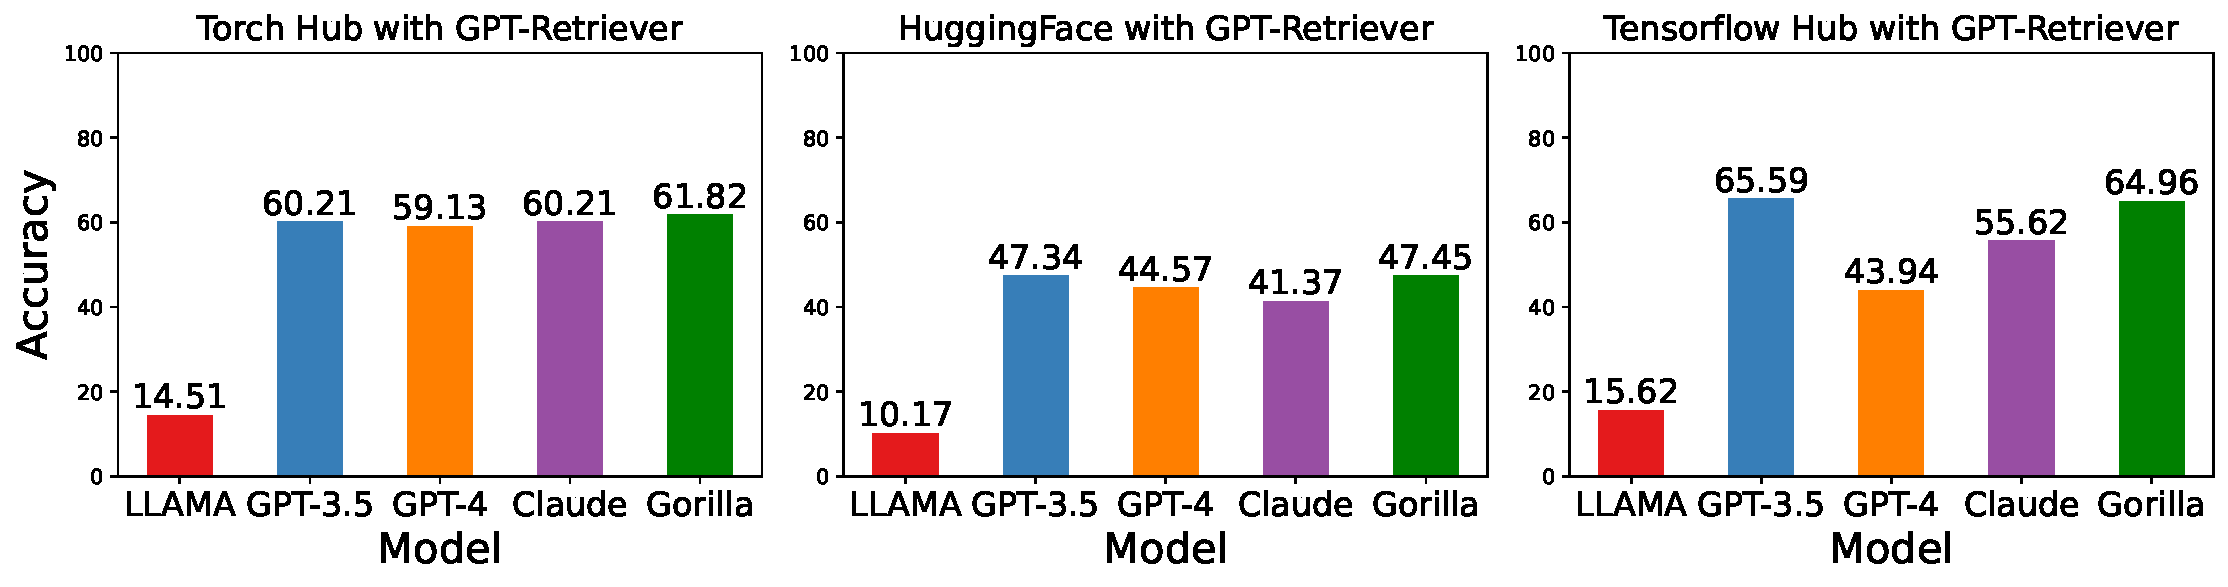
\includegraphics[width=\linewidth]{figures/grid_bars_GPT_Retrieval.pdf}
\caption{\footnotesize \textbf{Accuracy with GPT-retriever.} 
\oursmethod{} outperforms on Torch Hub and Hugging-Face while matching performance on Tensorflow Hub for all existing SoTA LLMs - closed source, and open source. }
\label{fig:images}
\end{figure}
We first demonstrate the results for the AST accuracy for different models. We present the results in Tab.~\ref{tab:llm_eval}. We test each model for different retriever settings defined above. We report the overall accuracy, the error by hallucination and the error by selecting wrong API call. Note that for TorchHub and TensorHub, we evaluate all the models using AST tree accuracy score. However, for HuggingFace, since the dataset is not exhaustive, for all the models except \oursmethod{}, we only check if they can provide the correct domain names. So this problem reduces to picking one of the multiple choices. 


\paragraph{Finetuning without Retrieval} In Tab.~\ref{tab:llm_eval} we show that lightly fine-tuned \oursmethod{} gets the state-of-the-art performance zero-shot over all the models, 20.43\% better than GPT-4 and 10.75\% better than ChatGPT. When compared to other open-source models LLAMA, the improvement is as big as 83\%. his suggests quantitatively, that finetuning is better than retrieval, at-least in our scope. 

In addition, we found that finetuning without retriever and putting ground truth retriever in evaluation time rarely helps the performance: 0.88\% worse in TensorHub and 0.97\% better in HuggingFace. If we put BM25 or GPT-Index as retriever, results will be significantly dropped: 21.50\% in Torch Hub and 47.57\% in HuggingFace. The result illustrates that adding a non-optimal retriever at test time will sometime misguide the model and result in more errors. We will discuss an interesting ablation on how finetuning with the retriever will help the performance in the next paragraph. 





\begin{table*}[h]
    \caption{\small \textbf{Evaluating LLMs on Torch Hub, HuggingFace, and Tensorflow Hub APIs}}
    \label{tab:llm_eval}
     \setlength{\tabcolsep}{10pt} % Default value: 6pt
    \begin{adjustbox}{width=\textwidth}
    \begin{tabular}{l c c c | c c c | c c c}
    \toprule
    
    LLM (retriever) & \multicolumn{3}{c}{TorchHub} & \multicolumn{3}{c}{HuggingFace} & \multicolumn{3}{c}{TensorFlow Hub} \\
    & overall $\uparrow$ & hallu $\downarrow$ & err $\downarrow$ & overall $\uparrow$ & hallu $\downarrow$ & err $\downarrow$ & overall $\uparrow$ & hallu $\downarrow$ & err $\downarrow$ \\
    \midrule
    LLAMA (0-shot) & 0 & 100 & 0 & 0.00 & 97.57 & 2.43 & 0 & 100 & 0 \\
    GPT-3.5 (0-shot) & 48.38 & 18.81 & 32.79 & 16.81 & 35.73 & 47.46 & 41.75 & 47.88 & 10.36 \\
    GPT-4 (0-shot) & 38.70 & 36.55 & 24.7 & 19.80 & 37.16 & 43.03 & 18.20 & 78.65 & 3.13 \\
    Claude (0-shot) & 18.81 & 65.59 & 15.59 & 6.19 & 77.65 & 16.15 & 9.19 & 88.46 & 2.33 \\
    \gorilla{} (0-shot) & \textbf{59.13} & \textbf{6.98} & 33.87 & \textbf{71.68} & \textbf{10.95} & 17.36 & \textbf{83.79} & \textbf{5.40} & 10.80 \\
    \midrule
    LLAMA (BM-25) & 8.60 & 76.88 & 14.51 & 3.00 & 77.99 & 19.02 & 8.90 & 77.37 & 13.72 \\
    GPT-3.5 (BM-25) & 38.17 & 6.98 & 54.83 & \textbf{17.26} & 8.30 & 74.44 & \textbf{54.16} & 3.64 & 42.18 \\
    GPT-4 (BM-25) & 35.48 & 11.29 & 53.22 & 16.48 & 15.93 & 67.59 & 34.01 & 37.08 & 28.90 \\
    Claude (BM-25) & 39.78 & 5.37 & 54.83 & 14.60 & 15.82 & 69.58 & 35.18 & 21.16 & 43.64 \\
    \gorilla{} (BM-25) & \textbf{40.32} & \textbf{4.30} & 55.37 & 17.03 & \textbf{6.42} & 76.55 & 41.89 & \textbf{2.77} & 55.32 \\
    \midrule
    LLAMA (GPT-Index) & 14.51 & 75.8 & 9.67 & 10.18 & 75.66 & 14.20 & 15.62 & 77.66 & 6.71 \\
    GPT-3.5 (GPT-Index) & 60.21 & 1.61 & 38.17 & 29.08 & 7.85 & 44.80 & \textbf{65.59} & 3.79 & 30.50 \\
    GPT-4 (GPT-Index) & 59.13 & 1.07 & 39.78 & 44.58 & 11.18 & 44.25 & 43.94 & 31.53 & 24.52 \\
    Claude (GPT-Index) & 60.21 & 3.76 & 36.02 & 41.37 & 18.81 & 39.82 & 55.62 & 16.20 & 28.17 \\
    \gorilla{} (GPT-Index) & \textbf{61.82} & \textbf{0} & 38.17 & \textbf{47.46} & \textbf{8.19} & 44.36 & 64.96 & \textbf{2.33} & 32.70 \\
    \midrule
    LLAMA (Oracle) & 16.12 & 79.03 & 4.83 & 17.70 & 77.10 & 5.20 & 12.55 & 87.00 & 0.43 \\
    GPT-3.5 (Oracle) & 66.31 & 1.60 & 32.08 & 89.71 & 6.64 & 3.65 & \textbf{95.03} & \textbf{0.29} & 4.67 \\
    GPT-4 (Oracle) & 66.12 & 0.53 & 33.33 & 85.07 & 10.62 & 4.31 & 55.91 & 37.95 & 6.13 \\
    Claude (Oracle) & 63.44 & 3.76 & 32.79 & 77.21 & 19.58 & 3.21 & 74.74 & 21.60 & 3.64 \\
    \gorilla{} (Oracle) & \textbf{67.20} & \textbf{0} & 32.79 & \textbf{91.26} & \textbf{7.08} & 1.66 & 94.16 & 1.89 & 3.94 \\
    \bottomrule
    \end{tabular}
    \end{adjustbox}
\end{table*}



\paragraph{Finetuning with Retrieval} We now discuss an interesting experiment on how finetuning language with retriever incorporated is helping the performance. The settings for this experiment are finetuning the base LLAMA with the prompt (instruction generated), reference API document (from golden-truth oracle), and the example output generated by GPT-4. In Tab.~\ref{tab:retrieve}, we can see that incorporating ground truth retriever in the finetuning pipeline achieves significantly better results 12.37\% better than training without retriever in Torch Hub and 23.46\% better in HuggingFace. However, we found that at evaluation time, current retrievers still have a big gap between the ground truth retriever: using GPT-Index at evaluation results in 29.20\% accuracy degradation, and using BM25 results in a 52.27\% accuracy degradation. Nevertheless, we can still conclude that with a better retriever, finetuning with retriever is still a better method to adopt while in another scenario, when a good retriever is not available, zero-shot finetuning might be the preferred choice.

\begin{table*}[h]
    \caption{\small \textbf{Comparison of retrieval techniques}
    }
    \label{tab:retrieve}
     \setlength{\tabcolsep}{10pt} % Default value: 6pt
    \begin{adjustbox}{width=\textwidth}
    \begin{tabular}{l cccc | cccc}
    \toprule
    & \multicolumn{4}{c}{\gorilla{} without Retriever} & \multicolumn{4}{c}{\oursmethod{} with Oracle retriever} \\ 
     % \cmidrule(lr){4-23}
     \midrule
    & zero-shot & BM25 & GPT-Index & Oracle & zero-shot & BM25 & GPT-Index & Oracle  \\
    \midrule
    Torch Hub (overall) $\uparrow$ & 59.13 & 37.63 & 60.21 & 54.83 & 0 & 40.32 & 61.82 & 67.20  \\
    HuggingFace (overall) $\uparrow$ & 71.68 & 11.28 & 28.10 & 45.58 & 0 & 17.04 & 47.46 & 91.26  \\
    TensorHub (overall)  $\uparrow$ & 83.79 & 34.30 & 52.40 & 82.91 & 0 & 41.89 & 64.96 & 94.16 \\
    \midrule
    Torch Hub (Hallu) $\downarrow$ & 6.98 & 11.29 & 4.30 & 15.59 & 100 & 4.30 & 0 & 0  \\
    HuggingFace (Hallu) $\downarrow$ & 10.95 & 46.46 & 41.48 & 52.77 & 99.67 & 6.42 & 8.19 & 7.08  \\
    TensorHub (Hallu) $\downarrow$ & 5.40 & 20.43 & 19.70 & 13.28 & 100 & 2.77 & 2.33 & 1.89\\
    \bottomrule
    \end{tabular}
    \end{adjustbox}
\end{table*}

\paragraph{Hallucination with LLM} One phenomenon we observe is that zero-shot prompting with LLMs (GPT-4/GPT-3.5) to call APIs results in dire hallucination errors. These errors, while diverse, commonly manifest in erroneous behavior such as the model invoking the "AutoModel.from\_pretrained(dir\_name)" command with arbitrary GitHub repository names. Surprisingly, we also found that in TorchHub, HuggingFace and TensorFlow Hub, GPT-3.5 has less hallucination errors than GPT-4. This finding is also consistent for the settings when various retrieving methods are provided: 0-shot, BM25, GPT-Index and the oracle. This might suggest that RLHF plays a central role in turning the model to be truthful. Additional examples and discussion are in Appendix.

\subsection{Test-Time Documentation Change}

\begin{figure}[t]
    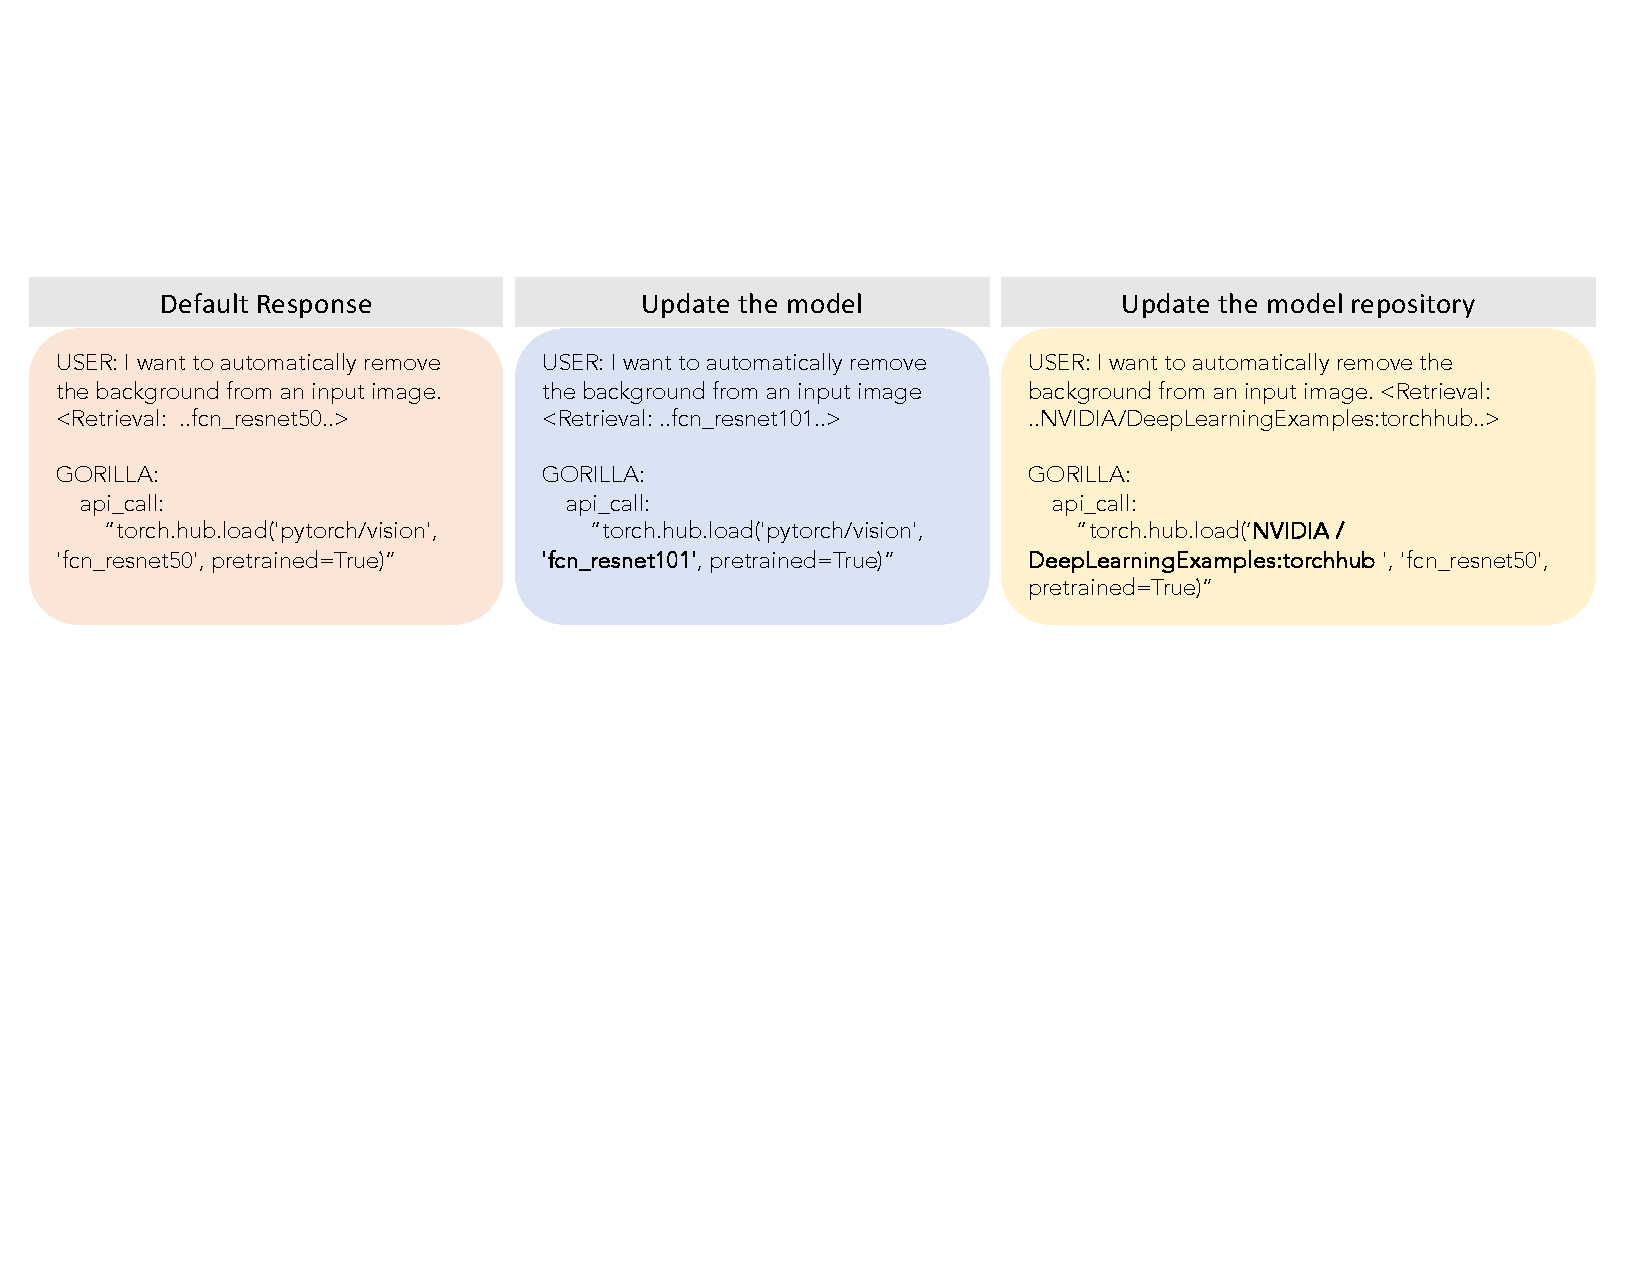
\includegraphics[width=\linewidth]{figures/docu.pdf}
\caption{\footnotesize \textbf{Gorilla's retriever\---aware training enables it to react to changes in the APIs.} The second column demonstrates changes in model \- upgrading FCN's ResNet\---50 backbone to ResNet\---101. The third column demonstrate changes in model registry from \texttt{pytorch/vision} to \texttt{NVIDIA/DeepLearningExamples:torchhub} }
\label{fig:docu}
\end{figure}


The rapidly evolving nature of API documentation presents a significant challenge for the application of LLMs in this field. These documents are often updated at a frequency that outpaces the re-training or fine-tuning schedule of LLMs, making these models particularly brittle to changes in the information they are designed to process. This mismatch in update frequency can lead to a decline in the utility and reliability of LLMs over time.

However, with the introduction of Gorilla's retriever-aware training, we can readily adapt to changes in API documentation. This novel approach allows the model to remain updated and relevant, even as the API documentation it relies on undergoes modifications. This is a pivotal advancement in the field, as it ensures that the LLM maintains its efficacy and accuracy over time, providing reliable outputs irrespective of changes in the underlying documentation.

For instance, consider the scenario illustrated in Figure 6, where the training of Gorilla has allowed it to react effectively to changes in APIs. This includes alterations such as upgrading the FCN's ResNet-50 backbone to ResNet-101, as demonstrated in the second column of the figure. This capability ensures that the LLM remains relevant and accurate even as the underlying models and systems undergo upgrades and improvements.
Furthermore, the third column in Figure 6 shows how Gorilla adapts to changes in the model registry from \texttt{pytorch/vision} to \texttt{NVIDIA/DeepLearningExamples:torchhub}. This reflects the model's ability to adjust to shifts in API sources, which is vital as organizations may change their preferred model registries over time.

In summary, Gorilla's ability to adapt to test-time changes in API documentation offers numerous benefits. It maintains its accuracy and relevance over time, adapts to the rapid pace of updates in API documentation, and adjusts to modifications in underlying models and systems. This makes it a robust and reliable tool for API calls, significantly enhancing its practical utility.



\subsection{API Call with Constraints}
We now focus on the language model's capability of understanding constraints. For any given task, which API call to invoke is typically a tradeoff between a multitude of factors. In the case of RESTFul APIs, it could be the cost of each invocation (\$), and the latency of response (ms), among others. Similarly, within the scope of ML APIs, it is desirable for \gorilla{} to respect constraints such as accuracy, number of learnable parameters in the model, the size on disk, peak memory consumption, FLOPS, etc. We present the underlying ablation study evaluating the ability of different models in zero-shot and with retrievers settings to respect a given accuracy constraint. This setting is best understood with an example. If the user were to ask for an Image classification model that achieves at least 80\% top-1 accuracy on the Imagenet dataset, then while both are classification models hosted by Torch Hub,    \texttt{ResNeXt-101 32x16d} with a top-1 accuracy of 84.2\% would be the right model whose API to call and not, say, \texttt{MobileNetV2} which has a top-1 accuracy of 71.88\%. 

\begin{table*}[h]
    \caption{\small \textbf{Evaluating LLMs on constraint-aware API invocations}
    }
    \label{tab:const}
    \begin{adjustbox}{max width=\textwidth}
    \begin{tabular}{l cccc|cccc|cccccc}
    \toprule
    & \multicolumn{4}{c}{GPT-3.5} & \multicolumn{4}{c}{GPT-4} & \multicolumn{4}{c}{\oursmethod{}}\\ 
     % \cmidrule(lr){4-23}
     \midrule
    & 0-shot & BM25 & GPT-Index & Oracle & 0-shot & BM25 & GPT-Index & Oracle & 0-shot & BM25 & GPT-Index & Oracle \\
    \midrule
    Torch Hub (overall) &  \textbf{73.94} & 62.67 & 81.69 & 80.98 & 62.67 & 56.33 & 71.11 & 69.01  & 71.83 & 57.04 & 71.83 & 78.16 \\
    Torch Hub (Hallu) &  19.01 & 30.98 & 14.78 & 14.08 & \textbf{15.49} & 27.46 & \textbf{14.08} & \textbf{9.15} & 19.71 & 39.43 & 26.05 & 16.90 \\
    Torch Hub (err) &  7.04 & 6.33 & 3.52 & 4.92 & 21.83 & 16.19 & 14.78 & 21.83 & 8.45 & 3.52 & 2.11 & 4.92 \\
    \midrule
    Accuracy const & 43.66 & \textbf{33.80} & \textbf{33.09} & 69.01 & 43.66 & 29.57 & 29.57 & 59.15 & \textbf{47.88} & 30.28 & 26.76 & 67.60\\
    \midrule
    & \multicolumn{4}{c}{LLAMA} & \multicolumn{4}{c}{Claude}\\ 
     % \cmidrule(lr){4-23}
     \midrule
      % \cmidrule{1-9}
    & 0-shot & BM25 & GPT-Index & Oracle & 0-shot & BM25 & GPT-Index & Oracle  \\
    % \midrule
    \cmidrule{1-9}
    Torch Hub (overall) &  0 & 8.45 & 11.97 & 19.71 & 29.92 & \textbf{81.69} & \textbf{82.39} & \textbf{81.69}\\
    Torch Hub (Hallu) &   100 & 91.54 & 88.02 & 78.87 & 67.25 & \textbf{16.19} & 15.49 & 13.38\\
    Torch Hub (err) &  0 & 0 & 0 & 1.4  & 2.81 & 2.11 & 2.11 & 4.92\\
    % \midrule
     \cmidrule{1-9}
    Accuracy const & 0 & 6.33 & 3.52 & 17.60 & 17.25 & 29.57 & 31.69 & \textbf{69.71}\\
    \bottomrule
    \end{tabular}
    \end{adjustbox}
\end{table*}

For Table~\ref{tab:const}, we filtered a subset of the Torch Hub dataset that had accuracy defined for at least one-dataset in its model card (65.26\% of TorchHub dataset in Table~\ref{tab:llm_eval}). We notice that with constraints, understandably, the accuracy drops across all models, with and without a retriever. \gorilla{} is able to match performance with the best-performing model GPT-3.5 when using retrievals (BM25, GPT-Index) and has the highest accuracy in the Zero-shot case. This highlights Gorilla's ability to navigate APIs while considering the trade-offs between different constraints. 


